\documentclass[10pt]{beamer}
\usefonttheme{professionalfonts,serif}
\def\newblock{\hskip .11em plus .33em minus .07em}
\usepackage[numbers,sort]{natbib}
\renewcommand{\rmdefault}{psbx}
\usepackage[utf8]{inputenc}
\usepackage[T1]{fontenc}
\usepackage{textcomp}
\usepackage{eulervm}

\usetheme{default}           % tips from David Blei
\useinnertheme{circles}
\useoutertheme{infolines}
\setbeamertemplate{headline}{}
\setbeamertemplate{navigation symbols}{}
\setbeamerfont{itemize/enumerate subbody}{size=\normalsize}
\setbeamerfont{itemize/enumerate subsubbody}{size=\normalsize}
\usecolortheme{seahorse}
\setbeamersize{text margin left=2mm,text margin right=2mm}

\graphicspath{{../../figures/}}

\definecolor{mypine}{rgb}{0.05,0.45,0.05}
\definecolor{mycyan}{rgb}{0.0,0.9,0.9}
\newcommand{\Red}{\textcolor{red}}
\newcommand{\Blue}{\textcolor{blue}}
\newcommand{\Green}{\textcolor{mypine}}
\newcommand{\PineGreen}{\textcolor{mypine}}
\newcommand{\Magenta}{\textcolor{magenta}}
\newcommand{\Cyan}{\textcolor{mycyan}}

\newcommand{\N}{\mathcal{N}}
\newcommand{\R}{\mathbb{R}}
\newcommand{\T}{{\scriptsize^{\top}}}
\newcommand{\D}{\mathcal{D}}
\newcommand{\F}{\mathcal{F}}
\newcommand{\E}{\mathbb{E}}
\newcommand{\V}{\mathbb{V}}
\newcommand{\M}{\mathcal{M}}
\newcommand{\KL}{\mathcal{KL}}
\newcommand{\cut}[1]{}
\newcommand{\trace}{\operatorname{trace}}

\newcommand{\bmu}{{\boldsymbol{\mu}}}
\newcommand{\btheta}{\boldsymbol{\theta}}
\newcommand{\bepsilon}{\boldsymbol{\epsilon}}
\newcommand{\balpha}{\boldsymbol{\alpha}}
\newcommand{\bbeta}{\boldsymbol{\beta}}
\newcommand{\bphi}{\boldsymbol{\phi}}
\newcommand{\bPhi}{\boldsymbol{\Phi}}
\newcommand{\bSigma}{\boldsymbol{\Sigma}}
\newcommand{\bpi}{\boldsymbol{\pi}}
\newcommand{\blambda}{\boldsymbol{\lambda}}

\newcommand{\argmax}{\operatorname{argmax}}
\newcommand{\argmin}{\operatorname{argmin}}
\newcommand{\ci}{{\bot\negthickspace\negthickspace\bot}} % conditional indep.
\newcommand{\neigh}{\operatorname{ne}}
\newcommand{\vectr}[2]{  \left[ \!\!\begin{array}{c} #1 \\
      #2 \end{array} \!\!\right]}
\newcommand{\deff}{\stackrel{\mathrm{def}}{=}}
\newcommand{\deldel}[2]{\frac{\partial #1}{\partial #2}}

\newcommand{\maketilde}{\raisebox{0.4ex}{\tiny $\sim$}}
\newcommand{\bfa}{\mathbf a}
\newcommand{\bfb}{\mathbf b}
\newcommand{\bfe}{\mathbf e}
\newcommand{\bff}{\mathbf f}
\newcommand{\bfk}{\mathbf k}
\newcommand{\bfm}{\mathbf m}
\newcommand{\bfn}{\mathbf n}
\newcommand{\bfp}{\mathbf{p}}
\newcommand{\bfs}{\mathbf s}
\newcommand{\bfu}{\mathbf u}
\newcommand{\bfx}{\mathbf x}
\newcommand{\bfy}{\mathbf y}
\newcommand{\bft}{\mathbf t}
\newcommand{\bfv}{\mathbf v}
\newcommand{\bfw}{\mathbf w}
\newcommand{\bfA}{\mathbf A}
\newcommand{\bfI}{\mathbf I}
\newcommand{\bfK}{\mathbf K}


\title{GP Marginal Likelihood and Hyperparameters}
\author{Carl Edward Rasmussen}
\date{October 18th, 2022}

\begin{document}

\begin{frame}
\titlepage
\end{frame}

\begin{frame}
\frametitle{Key concepts}
\begin{itemize}
\item We give an interpretation of the marginal likelihood in terms of
\begin{itemize}
\item a data fit
\item a complexity penalty
\end{itemize}
\item covariance functions can be parameterized using hyperparameters
\item hyperparameters can be fit by optimizing the marginal likelihood
\begin{itemize}
\item this is a form of model selection
\end{itemize}
\item Occam's razor is automatic and avoids overfitting
\end{itemize}
\end{frame}

\begin{frame}
\frametitle{The Gaussian process marginal likelihood}

Log marginal likelihood has a closed form
\[
\log Z_{|\bfy}\;=\;\log p(\bfy|\bfx,\mathcal{M}_i)\;=\;\Blue{-\frac{1}{2}\bfy
^\top [K+\sigma_n^2I]^{-1}\bfy}
-\Red{\frac{1}{2}\log|K+\sigma_n^2I|}-\frac{n}{2}\log(2\pi)
\]
and is the combination of a \Blue{data fit} term and \Red{complexity penalty}.
Occam's Razor is automatic.
\end{frame}


\begin{frame}
\frametitle{Hyperparameters: properties of covariance functions}

The covariance function which we have seen before
\[
k(x,x')\;=\;\exp(-\tfrac{1}{2}(x-x')^2),
\]
encodes that $f(x)$ and $f(x')$ have large covariance if $x$ is
\Blue{close to} $x'$, but it doesn't really quantify what is means by
\Blue{close to}?\\[1ex]

We can parameterize the covariance function using \Blue{hyperparameters} such as $\ell$, in
\[
k(x,x')\;=\;\exp\big(-\frac{(x-x')^2}{2\ell^2}\big).
\]

\Blue{Learning} in Gaussian process models involves finding
\begin{itemize}
\item the form of the covariance function, and
\item any unknown (hyper-) parameters $\theta$.
\end{itemize}

\end{frame}

\begin{frame}
\frametitle{Example: Fitting the length scale parameter}

Parameterized covariance function: $k(x,x') =
v^2\exp\big(-\displaystyle\frac{(x-x')^2}{2\ell^2}\big)
+\sigma_\mathrm{noise}^2\delta_{xx'}$.
\vskip-4mm
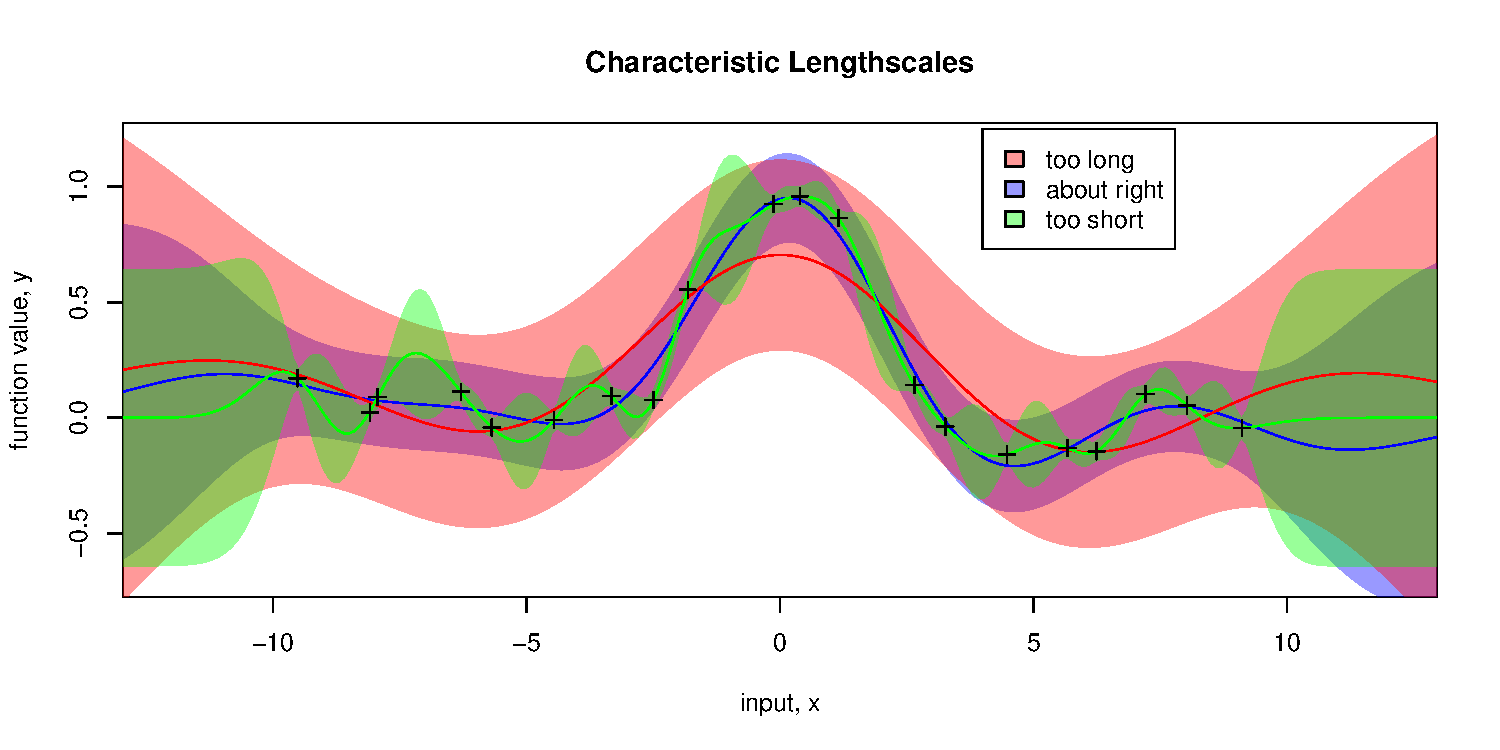
\includegraphics[width=\textwidth]{longshort2}
\vskip-4mm
The mean posterior predictive function is plotted for 3 different
length scales (the blue curve corresponds to optimizing the marginal
likelihood). \Red{Notice, that an almost exact fit to the data can be
achieved by reducing the length scale -- but the marginal likelihood
does not favour this!}
\end{frame}


\begin{frame}
\frametitle{How can Bayes rule help find the right model complexity? 
  Marginal likelihoods and Occam's Razor}
\centerline{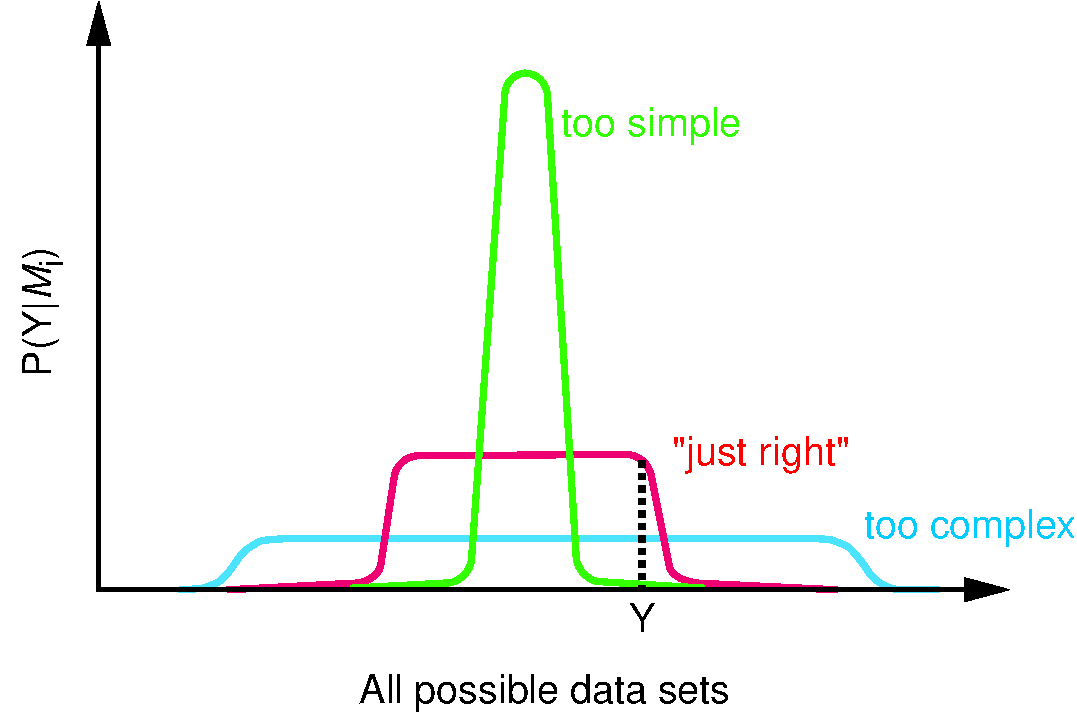
\includegraphics[width=0.85\textwidth]{ockham}}
\end{frame}


\begin{frame}
\frametitle{An illustrative analogous example}
Imagine the simple task of fitting the variance, $\sigma^2$, of a zero-mean
Gaussian to a set of $n$ scalar observations.

\centerline{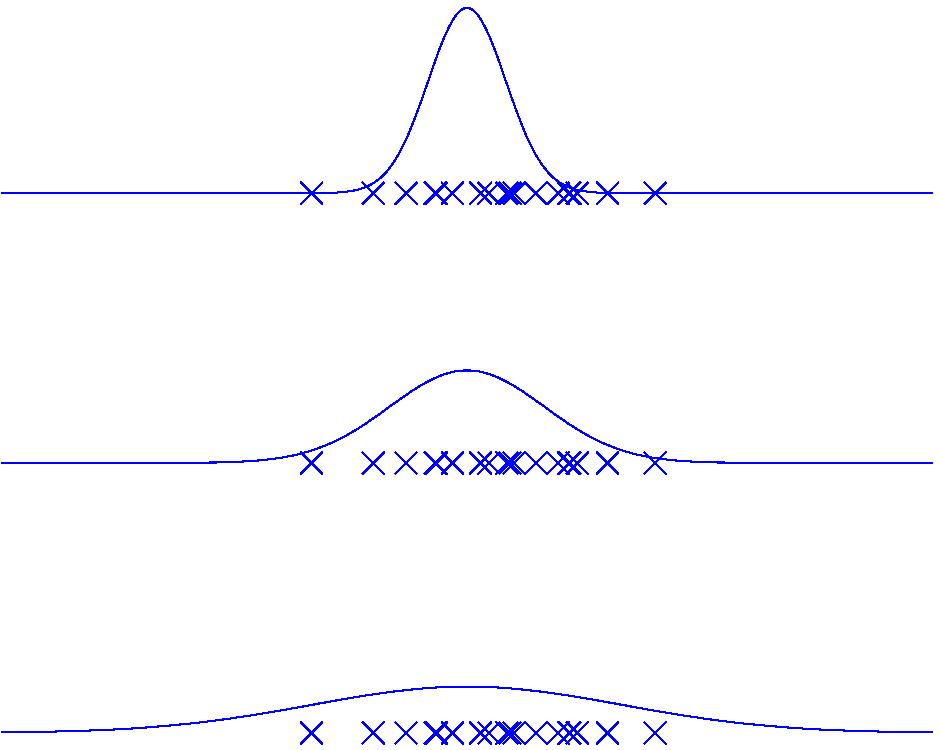
\includegraphics[width=0.6\textwidth]{sgex}}

The log likelihood is $\log p(\bfy|\mu,\sigma^2) =
\Blue{-\tfrac{1}{2}{\bf y}^\top I{\bf y}/\sigma^2} \Red{-\tfrac{1}{2}\log|I\sigma^2|}-
\tfrac{n}{2}\log(2\pi)$ 

\end{frame}
\end{document}
